\appendix
%% Правка оформления ссылок на приложения:
%http://tex.stackexchange.com/questions/56839/chaptername-is-used-even-for-appendix-chapters-in-toc
%http://tex.stackexchange.com/questions/59349/table-of-contents-with-chapter-and-appendix
%% требует двойной компиляции
\addtocontents{toc}{\def\protect\cftchappresnum{\appendixname{} }%
\setlength{\cftchapnumwidth}{\widthof{\cftchapfont\appendixname~Ш\cftchapaftersnum}}%
}
%% Оформление заголовков приложений ближе к ГОСТ:
\sectionformat{\chapter}[display]{% Параметры заголовков разделов в тексте
    label=\chaptertitlename\ \thechapter,% (ГОСТ Р 2.105, 4.3.6)
    labelsep=20pt,
}
\renewcommand\thechapter{\Asbuk{chapter}} % Чтобы приложения русскими буквами нумеровались
\chapter{Единицы измерения потока фотонов}
В области синхротронного излучения приняты специфические единицы измерения потока фотонов:
\begin{equation}
	\Phi = \cfrac{\gamma}{\textup{сек} \cdot 0.1\%\textup{bw} \cdot \textup{мм}^2}
\end{equation}
Для удобства пользователей этого излучения, была введено необычное единица $0.1\%\textup{bw}$, что можно интерпретировать следующим образом, --- это количество фотонов попавшее в полосу пропускания шириной $0.1\%$ на некоторой фиксированной энергии гамма-квантов, т.е., например, для энергии $1000 \textup{eV}$ ширина полосы будет в диапазоне $999,5 - 1000,5 \textup{eV}$. Данная единица была введена, для удобства оценок потоков, после прохождения излучения через кристаллические монохроматоры и решёточные монохроматоры, полосы пропускания которых как раз составляют порядка $10^{-3} - 10^{-4}$. 

Иногда возникает потребность, для удобства, перевести эти единицы, например, к следующему виду:
\begin{equation}
\Phi = \cfrac{\gamma}{\textup{сек} \cdot \textup{eV} \cdot \textup{мм}^2}
\end{equation} 
Сделать это можно следующим образом, необходимо поточено умножить спектральное распределение на множитель $\cfrac{0.1 \% \cdot E_{ph}}{1\textup{eV}}$, что даст необходимые единицы измерения. Далее, спектр можно привести к:
\begin{equation}
\Phi = \cfrac{W}{\textup{eV} \cdot \textup{мм}^2},
\end{equation} 
Так спектральное распределение легко интегрировать, чтобы получить, например, полную плотность мощности излучения и делать оценки тепловых нагрузок на оптические элементы.
\chapter{Краткий обзор дифракции на кристаллах}
В этой главе мы кратко дадим основные результаты кинетической и динамической теории дифракции. Основные кристаллы используемы на источниках синхротронного излучения --- это $Si$ (кремний), $C$ (алмаз) и реже $Ge$ (германий). Виду кубической кристаллической решётки эти кристаллы относительно просты при рассмотрение динамики отражение и преломления на кристаллических плоскостях. Для нас важны такие свойства кристаллов, как способность преобразовать относительно широкой спектр ондуляторного излучения в излучение с относительной монохроматичностью до $\Delta E/ E \sim 10^{-4}$. Также мы дадим основную информация по поглощательным способностям кристаллов
\section{Симметричное брэгговское отражение от идеально кристалла}
Длины волн, которые отвечают резонансу при отражении падающего под углом $\theta$ к плоскости кристалла излучения, даётся законом Брэгга:  
%пропорциональный $\gamma / nN$, где $n$ --- номер гармоники излучения, $N$ --- число периодов ондулятора, а $\gamma$ --- гамма фактор релятивистского электрона
\begin{equation}
	m\lambda = 2d\sin\theta,
\end{equation}
где $d$ --- расстояние между плоскостями от которых происходит отражение, $m$ --- некоторое положительно целое число. Однако динамическая и кинематическая теории дифракции уточнаю данные результат и вносят конечную угловую и/или по энергии ширину, в которую кристалл может принять излучение, а также некоторый сдвиг, относительно предполагаемого брэгговского угла.  Кривая, которая описывает отражательную способность кристалла, называется кривой Дарвина, именно она определяет угловой и/или энергетический акцептанс излучения. На рис.~\ref{fig:bragg_R} показаны характерные кривые отражение для алмаза и кремния. 
\begin{figure}
	\centering  
	\begin{minipage}{0.49\textwidth}
		\centering
		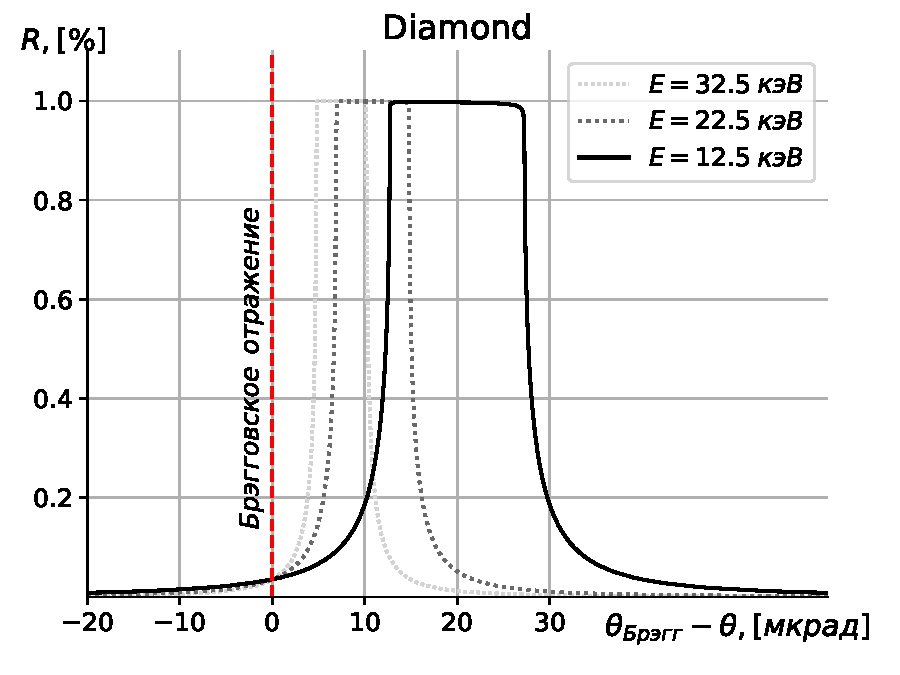
\includegraphics[width=\textwidth]{pic/Diamond_bragg_R.pdf}
		\caption{Кривая брегга для алмаза на разных энергиях}
		\label{fig:bragg_R}
	\end{minipage}\hfill
	\begin{minipage}{0.49\textwidth}
		\centering
		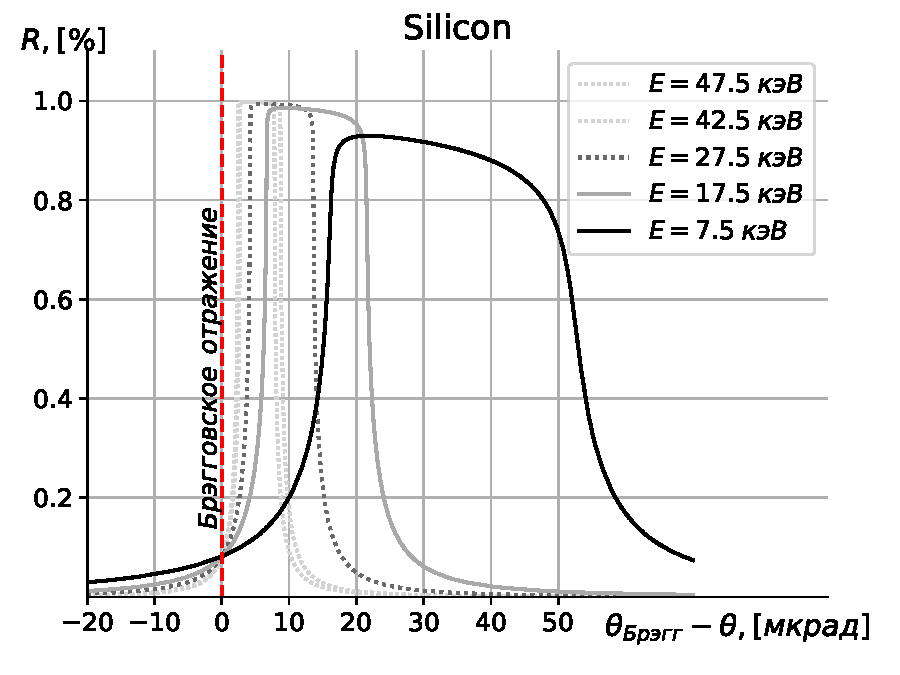
\includegraphics[width=\textwidth]{pic/Silicon_bragg_R.pdf}
		\caption{Кривая брегга для кремния на разных энергиях}
		\label{fig:bragg_T}
	\end{minipage}    
\end{figure}
По ним видно, чем больше энергия подающего пучка излучения, тем  кривая уже и ближе к даваемому законом брэгга углу. При расчёте кристаллов монохроматоров этот факт необходимо учитывать, для эффективной работы кристалла и уменьшения тепловых нагрузок, угловая расходимость кристалла должна входить в акцептанс кристалла, иначе излучение поглотится в кристалле, что крайне нежелательно. Кривые ассиметричны по правому краю, теория дифракции объясняет данный факт большим поглощением на низких энергиях.

В целом, данной информации достаточно, чтобы иметь первое представление о разработке оптических трактов синхротронного излучения. Для дальнейшего чтения и углубления знаний в данном вопросе могут быть полезны следующие книги \cite{als2011elements}, \cite{authier2006dynamical}.

\section{Поглощательные способности кристаллов}
Одним из полезных применений кристаллов в рентгеновском диапазоне есть их фильтрующая способность, отрезать низкие энергии, в особенности для алмазных кристаллов, которые, по мимо всего, имеют хорошую теплопроводность, что способствуют быстрому теплоотводу. На рис.~\ref{fig:bragg_T} представлена кривая поглощения 100 мкм кристалла алмаза. Подобные кристаллы устанавливают перед первыми оптическими элементами, что в значительной степени снижает тепловые нагрузки, подавляя низшие гармоники, в нашем случае ондуляторного излучения. 
\chapter{Дополнительные графики} \label{AppendixA}

\chapter{Примеры программного кода} \label{AppendixB}

\section{Подраздел приложения}\label{AppendixB1}

\normalsize% возвращаем шрифт к нормальному
